%%=============================================================================
%% Inleiding
%%=============================================================================

\chapter{Inleiding}
\label{ch:inleiding}

%De inleiding moet de lezer alle nodige informatie verschaffen om het onderwerp te begrijpen zonder nog externe werken te moeten raadplegen \autocite{Pollefliet2011}. Dit is een doorlopende tekst die gebaseerd is op al wat je over het onderwerp gelezen hebt (literatuuronderzoek).

%Je verwijst bij elke bewering die je doet, vakterm die je introduceert, enz. naar je bronnen. In \LaTeX{} kan dat met het commando \texttt{$\backslash${textcite\{\}}} of \texttt{$\backslash${autocite\{\}}}. Als argument van het commando geef je de ``sleutel'' van een ``record'' in een bibliografische databank in het Bib\TeX{}-formaat (een tekstbestand). Als je expliciet naar de auteur verwijst in de zin, gebruik je \texttt{$\backslash${}textcite\{\}}.
%Soms wil je de auteur niet expliciet vernoemen, dan gebruik je \texttt{$\backslash${}autocite\{\}}. Hieronder een voorbeeld van elk.

%\textcite{Knuth1998} schreef een van de standaardwerken over sorteer- en zoekalgoritmen. Experten zijn het erover eens dat cloud computing een interessante opportuniteit vormen, zowel voor gebruikers als voor dienstverleners op vlak van informatietechnologie~\autocite{Creeger2009}.








%--------------------------------------

\section{Stand van zaken}
\label{sec:stand-van-zaken}
Bedrijven kunnen tegenwoordig niet zonder IT-infrastructuur. Deze infrastructuur kan zeer uitgebreid en complex zijn. Bovendien moet het ook nog schalen naarmate het bedrijf groeit. Als systeembeheerder heb je diverse taken waaronder zaken zoals incident management en het volgen van de laatste technologische trends en bedreigingen. Het opzetten en configureren van de zoveelste identieke server is dus een groot tijd- en geldverlies. Daarom werden configuration management tools in het leven geroepen. De eerst bekende tool was Puppet. Deze technologie stelde ons in staat om configuraties van servers als het ware te programmeren. Eens de gewenste configuratie geprogammeerd is kunnen extra gelijkaardige servers veel sneller opgezet worden. De systeembeheerders van vroeger zijn nu meer een meer DevOp geworden. Dit zijn dus mensen die zich niet enkel bezig houden met systeembeheer maar ook met software-ontwikkeling. Ze ontwikkelen als het ware de configuraties van servers. Puppet is daar altijd al marktleider in geweest. Dit is ook te zien is op figuur \ref{fig:popcon_everybody}. Maar daar komt nu verandering in. Er is de laatste jaren meer concurentie op de markt gekomen waaronder relatief bekenden zoals Salt en Chef. 
Echter,  \'e\'en van deze nieuwe CMT 's doet het opvallend beter op gebied van populariteit en dat is Ansible inc. Zoals op de grafiek te zien is heeft Ansible in 2015 de leiding genomen. Het was ook bovendien in dat jaar dat Ansible werd vernoemd door multinationals zoals Gartner die Ansible vernoemde in een artikel over  'Cool Vendors in DevOps' \autocite{coolvendors}. Verder was het Red Hat die aankondigde dat er een akkoord was om Ansible over te nemen \autocite{redhatovername}. Voorlopig laat volgens de populariteits-grafiek van Debian \ref{fig:popcon_everybody} Ansible zijn concurenten ver achter zich. Maar wie zijn Puppet en Ansible nu eigenlijk?

\begin{figure}
  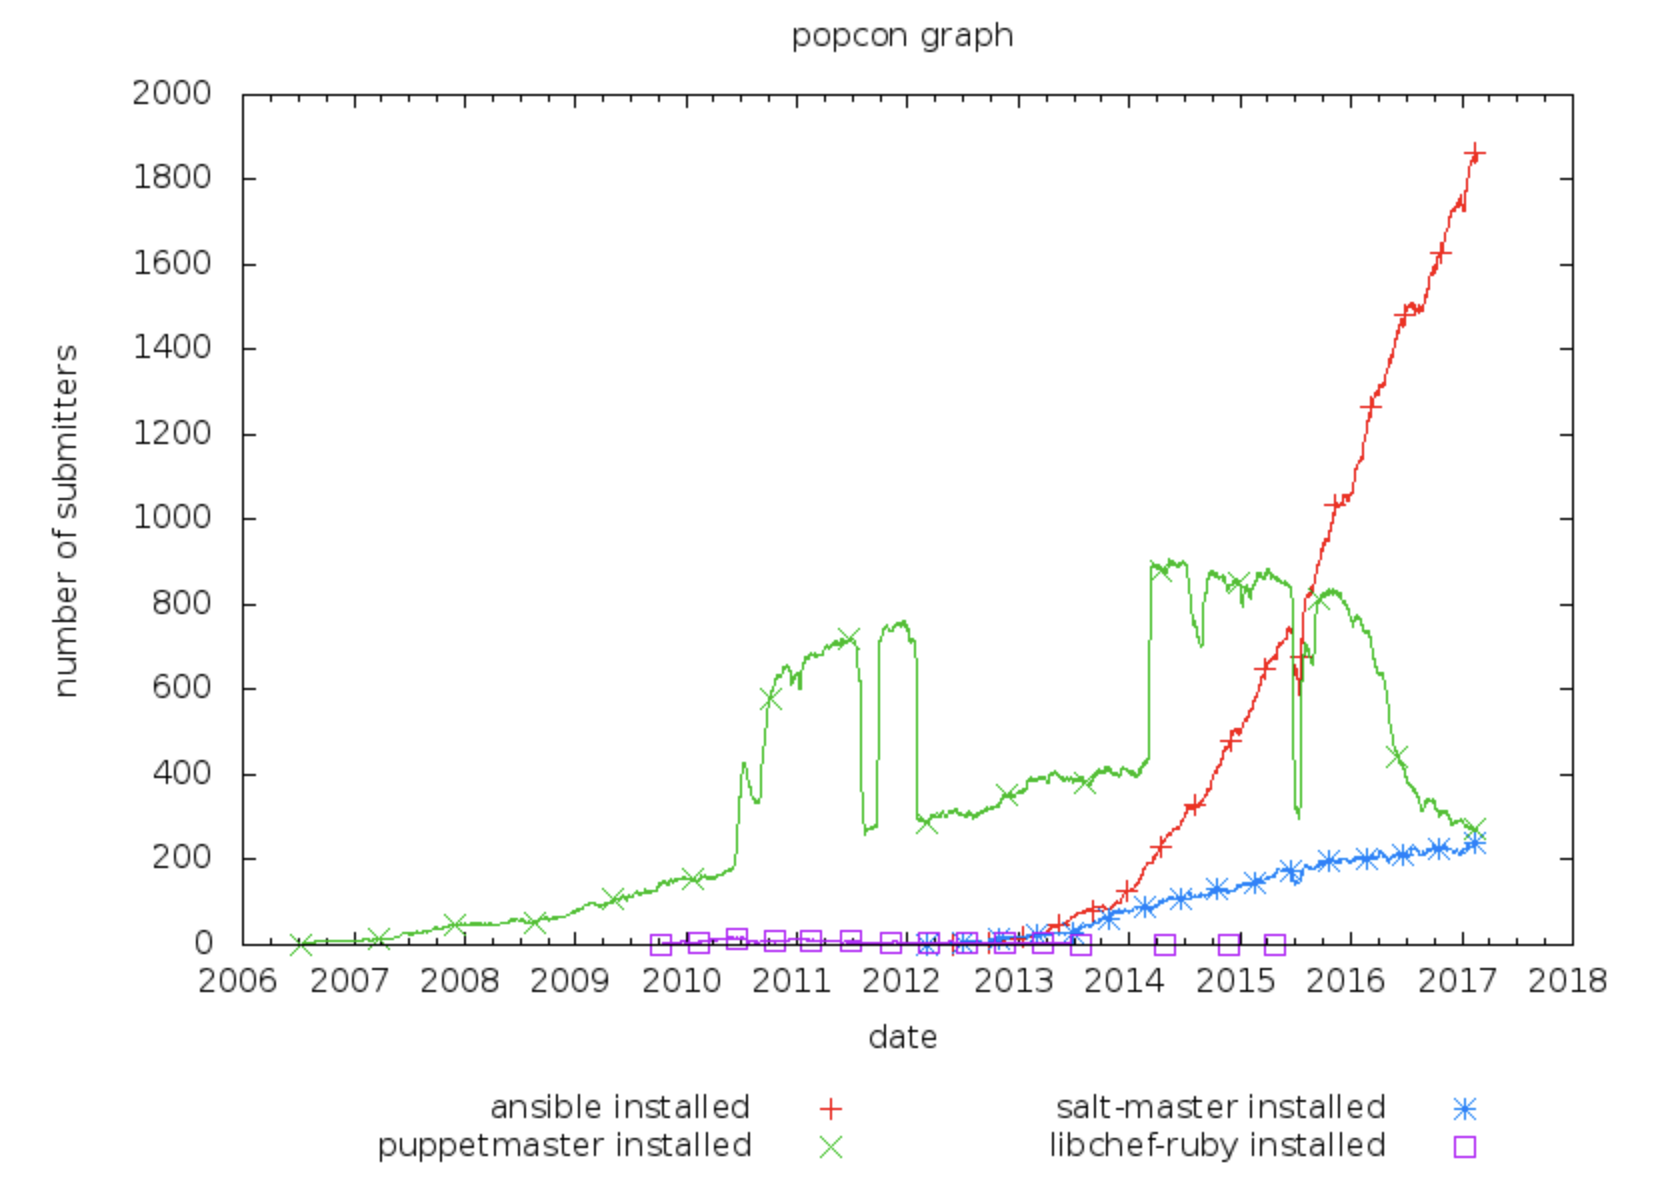
\includegraphics[width=\linewidth]{img/popcon_everybody.png}
  \caption{Deze grafiek toont het aantal keren dat een bepaald softwarepakket ge\"{\i}nstalleerd is op een debian distributie. \autocite{popcon}}
  \label{fig:popcon_everybody}
\end{figure}

\subsection{Profiel van Puppet}

Puppet werd ontwikkeld in 2005 met als doel het automatiseren van data centers. \autocite{puppetfaq}. Om dit te kunnen verwezelijken maakt puppet gebruik van  het server/client model. De server word hierbij de puppetmaster genoemd. Dit kan er   \'e\'en of meerderen zijn. De client wordt de puppetagent genoemd. Zowel op de master als op de client dient puppet ge\'enstalleerd te zijn om te kunnen functioneren. Tussen de master en de client bestaat er een vertrouwensrelatie die onderhouden wordt door certificaten. Ook de puppetmaster is verantwoordelijk voor het verlenen van deze certificaten. Al deze communicatie verloopt bovendien via het HTTPS-protocol. Pas als dit alles in orde is kan Puppet pas aan de configuratie beginnen. De code die je schrijft wordt een manifest genoemd. Wanneer een puppetagent wilt controleren of hij nog up-to-date is zal hij een catalog aanvragen bij de puppetmaster. Een dergelijke catalog is een manifest gecompiled door de puppetmaster en is quasi uniek voor meeste hosts. Tenzij beide hosts zelf ook identiek zijn. Hierbij worden rekening gehouden met verschillende zaken waaronder de functie van de puppetagent maar ook de distributie van het besturingssysteem \autocite{puppetlanguagecatalog}. Vervolgens controleerd de puppetagent voor zichzelf of er verschillen zijn tussen zijn configuratie en de staat die beschreven staat in de catalog. Indien er afwijkingen zijn worden deze ook automatisch opgelost.\autocite{puppetdoc}


\subsection{Profiel van Ansible}
Ansible is opgericht door Michael DeHaan, iemand die zeer vertrouwd was met Puppet \autocite{ansiblefordevops}. Hij vond dat bedrijven die Puppet gebruikten moeilijkheden ondervonden op gebied van eenvoud en automatisatie. Daarom is hij samen met Sa{\"\i}d Ziouani Ansible Inc. gestart. 
Ansible maakt niet gebruik van agents. Dit betekend dat de ansibleserver enkel het IP-adres en het wachtwoord dient te weten van de servers die hij moet configureren. De code die beschrijft hoe deze servers geconfigureerd moeten worden zijn geschreven in YAML en de verzameling van al deze configuraties word een playbook genoemd. Wanneer Ansible een bepaalde server wenst te configureren wordt dit standaard verzorgt door het SSH-protocol. Het authenticeren kan op verschillende manieren. Er wordt aangeraden om gebruik te maken van een SSH-key, wat het eenvoudigst is. Maar ook andere middelen zoals een ordinair wachtwoord of het kerberos-protocol worden ondersteunt. Eens de verbinding tot stand is gebracht verstuurt Ansible modules naar de te configureren server. Deze modules worden vervolgens uitgevoerd en weer verwijderd. \autocite{ansibledoc}


%% TODO: deze sectie (die je kan opsplitsen in verschillende secties) bevat je
%% literatuurstudie. Vergeet niet telkens je bronnen te vermelden!





\section{Opzet van deze bachelorproef}
\label{sec:opzet-bachelorproef}

In dit onderzoek vallen kleinere CMT's zoals Chef en Salt buiten de scope en zal er bijgevolg de focus gelegd worden op Puppet en Ansible. Dit onderzoek vind plaats binnen de VRT. Momenteel wordt er gebruik gemaakt van Puppet maar deze voldoet niet aan de verwachtingen van de bussiness en daarom is er dan ook besloten geweest om de huidige puppet-infrastructuur te vervangen door Ansible.
Deze bachelorproef wilt een hulp bieden aan bedrijven die dezelfde overstap overwegen. Ansible stijgt drastisch in populariteit, zoveel is zeker. Maar het is echter niet de eerste keer dat er een hype ontstond rond een onderwerp dat vervolgens gigantische teleurstelling veroorzaakte bij een community. Inmiddels heeft Ansible zich al kunnen bewijzen door possitieve analyses te krijgen van RedHat en Gartner. Maar is het zo dat Ansible het beter is dan Puppet die inmiddels al 12 jaar ervaring heeft?




\section{Probleemstelling en Onderzoeksvragen}
\label{sec:onderzoeksvragen}

%% TODO:
%% Uit je probleemstelling moet duidelijk zijn dat je onderzoek een meerwaarde
%% heeft voor een concrete doelgroep (bv. een bedrijf).
%%
%% Wees zo concreet mogelijk bij het formuleren van je
%% onderzoeksvra(a)g(en). Een onderzoeksvraag is trouwens iets waar nog
%% niemand op dit moment een antwoord heeft (voor zover je kan nagaan).


%% TODO: Het is gebruikelijk aan het einde van de inleiding een overzicht te
%% geven van de opbouw van de rest van de tekst. Deze sectie bevat al een aanzet
%% die je kan aanvullen/aanpassen in functie van je eigen tekst.

De overschakeling van Puppet naar Ansible is geen kleine stap die ongetwijfeld voor complicaties zal zorgen. Daarom weet men best op voorhand wat er te wachten staat en wat voordelen en nadelen kunnen zijn aan deze overschakeling. Daarom zal er in dit onderzoek verschillende relevante zaken onderzocht worden. Deze kunnen opgedeeld worden in drie grote categorie\'en. 
\subsection{Wat zijn de technische voor-en nadelen van Puppet en Ansible?}

In de eerste categorie zal er een vergelijkende studie plaatsvinden waarbij technische aspecten zoals performantie, schaalbaarheid in veiligheid vergeleken worden. Onder performantie wordt verstaan de tijd die het kost tot het bekomen van een consistente staat. Dit wordt onderzocht in twee situaties, namelijk als er nog geen configuratie aanwezig is en wanneer de server reeds geconfigureerd is maar enkele aanpassingen moeten doorgevoerd worden. Een tweede aspect van deze categorie is schaalbaarheid. Onder schaalbaarheid wordt verstaan: het vermogen om grote vraag te verwerken zonder kwaliteit te verliezen \autocite{informit}. We zullen monitoren hoe Ansible en Puppet hun resources verdelen bij een toenemende drukte, hier onder de vorm van meer servers en uitgebreidere configuraties. Voor het laatste aspect van deze eerste categorie, veiligheid, zal er in de eerste plaats een literatuurstudie plaatsvinden met onderzoek naar welke veilig- heidsproblemen reeds gekend zijn en wat de best practises zijn


\subsection{Wat zijn de redenen van een omschakeling}

Dit gedeelte van het onderzoek zal zich meer op sociaal vlak afspelen. De verantwoordelijken binnen VRT voor de overstap van Puppet naar Ansible zullen een paar vragen voorgelegd krijgen, al dan niet tijdens een informeel gesprek. Op deze manier zal getracht worden de drijfveren achter hun beslissing tot overstap bloot te leggen.

\subsection{Wat is het verloop van een dergelijk transitperiode}

De omschakeling bij VRT is reeds begonnen op het moment van het schrijven van dit onderzoeksvoorstel en zal nog steeds bezig zijn tijdens het onderzoek zelf. Problemen die bij de vervanging van Puppet door Ansible optreden zullen gerap- porteerd worden en er zal onderzocht worden waarom deze optraden. Al dan niet gevonden oplossingen zullen beschreven en uitgelegd worden. Welke incidenten zich zullen voordoen, valt uiteraard moeilijk te voorspellen. Bijgevolg is de grootte van deze sectie moeilijk in te schatten.

%%In Hoofdstuk~\ref{ch:methodologie} wordt de methodologie toegelicht en worden de gebruikte onderzoekstechnieken besproken om een antwoord te kunnen formuleren op de onderzoeksvragen.

%% TODO: Vul hier aan voor je eigen hoofstukken, één of twee zinnen per hoofdstuk

%%In Hoofdstuk~\ref{ch:conclusie}, tenslotte, wordt de conclusie gegeven en een antwoord geformuleerd op de onderzoeksvragen. Daarbij wordt ook een aanzet gegeven voor toekomstig onderzoek binnen dit domein.

